\documentclass[12pt]{report}
\usepackage[a4paper, left=3.17cm, right=3.17cm, top=2.54cm, bottom=2.54cm]{geometry}
\usepackage[T1]{fontenc}
\usepackage{mathptmx}
\usepackage{amsmath}
\usepackage{amsfonts}
\usepackage{chemformula}
\usepackage{multicol}
\usepackage{multirow}
\usepackage{listings}

\usepackage{xcolor}  % for syntax highlighting colors

\documentclass{article}
\usepackage{listings}
\usepackage{xcolor}

\definecolor{lightgray}{gray}{0.95}

\lstdefinestyle{matlabStyle}{
  language=Matlab,
  backgroundcolor=\color{lightgray},
  basicstyle=\ttfamily\small,
  keywordstyle=\color{blue}\bfseries,
  commentstyle=\color{gray}\itshape,
  stringstyle=\color{red},
  numbers=left,
  numberstyle=\tiny\color{gray},
  stepnumber=1,
  numbersep=8pt,
  frame=single,
  breaklines=true,
  showstringspaces=false,
  captionpos=b
}

        
\usepackage{tabularx,booktabs}
\newcolumntype{C}{>{\centering\arraybackslash}X} % centered version of "X" type
\usepackage[linesnumbered,ruled,vlined]{algorithm2e}
\usepackage{comment}
\usepackage{array}
\newcolumntype{P}[1]{>{\centering\arraybackslash}p{#1}}
\usepackage{cite}
\usepackage[colorlinks, linkcolor=black, anchorcolor=black, citecolor=black]{hyperref}
\usepackage{graphicx}
\setlength{\parskip}{0.5em}
\title{Place Your Project Title at Here}
%\author{\textup{Qi YUAN}}


%copyright at footer
\usepackage{fancyhdr}
\fancyhf{}
\rfoot{%
  \footnotesize
  \textcopyright~Dept. of Computer Science and Engineering, GUB\\

 }
%\pagestyle{fancy}


\begin{document}
    \input{title/title.tex}
    \tableofcontents
  
% Chapter 1 starting here.....    
\newpage
\chapter{Introduction}

\section{Overview}
This project is about simulating how errors happen during data transmission using line coding. Line coding is a method used to send digital data as signals from one place to another. We will create a simple program that shows how data can get changed or corrupted when errors occur in transmission.

\section{Objectives}
\begin{itemize}

\item  To understand what line coding is and how it works.
\item To simulate how errors can occur during data transmission.
\item To show how original data changes after errors happen.


\end{itemize}

\section{Features}
\begin{itemize}
\item  Simulates line coding with random error generation.
\item  Shows both original and received data for comparison.

\item Supports basic line coding types like NRZ, RZ, Manchester.

\item Easy-to-use interface for testing and learning.
\end{itemize}

\section{ Technical Requirements}
\begin{itemize}
\item  Programming Language:  C (Mathlab)

\item Platform: PC or Laptop with basic specifications


    \end{itemize}
\end{itemize}
\section{Discussion}
Line coding is very important in digital communication systems. This project helps us learn how small errors in transmission can change the whole message. With this simulation, we can see how data gets affected and why error detection and correction are important. It is useful for students to understand the basics of communication systems.
% Chapter 1 ends here.....    




% Chapter 2 starting here.....    
\newpage
\chapter{Design/Development/Implementation of the Project}

\section{Introduction}
This chapter explains how the project was designed, developed, and implemented. We created a simple program that shows how line coding works and how errors affect data. It helps students understand how digital data is sent and what problems can happen during transmission.
\subsection{Features:}

\item . Shows how binary data is sent using line coding.
\item . Supports line coding types like NRZ, RZ, and Manchester.

\item . Easy to understand with simple output display.

\begin{itemize}
\end{itemize}
\end{enumerate}


\section{Project Details}
The project takes input binary data from the user. It applies a selected line coding method to convert the data into signals. Then, it adds some random noise (errors) to the signal. Finally, it shows the changed data and compares it with the original
\begin{center}

\end{center}


\subsection{System Architecture}
The system architecture is simple and modular:
\begin{itemize}
     
\item Input Stage:
User enters the binary data (like 1011001).
\item Line Coding Stage:
The program converts the data into signal format using line coding (NRZ, RZ, etc.).
\item Error Simulation Stage:
Random bits are changed to simulate errors.
\item Output Stage:
The program displays both original and received data and highlights any changes.

\end{itemize}

\section{Implementation}

\subsection{Code}
The project is implemented using  Mathlab
\section{Mathlab code}
\begin{lstlisting}[style=matlabStyle, caption={}]

%% Line Coding Error Simulator with User Interface
clc; clear; close all;
disp('=== LINE CODING ERROR SIMULATOR ===');
fprintf('\n');
%% User Input Section
% 1. Select line coding scheme
fprintf('Available Line Coding Schemes:\n');
fprintf('1. Unipolar NRZ\n');
fprintf('2. Polar NRZ\n');
fprintf('3. Manchester\n');
fprintf('4. AMI\n');
scheme_idx = input('Select coding scheme (1-4): ');

% 2. Set simulation parameters
N = input('Enter number of bits to transmit (e.g., 1000): ');
bit_rate = input('Enter bit rate in bps (e.g., 1000): ');
Fs = input('Enter sampling frequency in Hz (e.g., 20000): ');
SNR_dB = input('Enter SNR values as array [start:step:end] (e.g., 0:2:20): ');

% Validate input
if scheme_idx < 1 || scheme_idx > 4
    error('Invalid coding scheme selection!');
end
coding_schemes = {'Unipolar NRZ', 'Polar NRZ', 'Manchester', 'AMI'};
selected_scheme = coding_schemes{scheme_idx};

fprintf('\n=== Simulation Parameters ===\n');
fprintf('Coding Scheme: %s\n', selected_scheme);
fprintf('Number of bits: %d\n', N);
fprintf('Bit rate: %d bps\n', bit_rate);
fprintf('Sampling frequency: %d Hz\n', Fs);
fprintf('SNR range: %s dB\n', mat2str(SNR_dB));
fprintf('\n');
%% Generate Random Binary Data
data = randi([0 1], 1, N);

%% Simulation
BER_results = zeros(1, length(SNR_dB));
encoded_signals = cell(1, length(SNR_dB));
noisy_signals = cell(1, length(SNR_dB));

for snr_idx = 1:length(SNR_dB)
    % Encoding
    switch scheme_idx
        case 1 % Unipolar NRZ
            encoded_signal = repelem(data, Fs/bit_rate);
        case 2 % Polar NRZ
            encoded_signal = repelem(data*2 - 1, Fs/bit_rate);
        case 3 % Manchester
            manchester = [];
            for bit = data
                if bit == 1
                    manchester = [manchester ones(1,Fs/(2*bit_rate)) -ones(1,Fs/(2*bit_rate))];
                else
                    manchester = [manchester -ones(1,Fs/(2*bit_rate)) ones(1,Fs/(2*bit_rate))];
                end
            end
            encoded_signal = manchester;
        case 4 % AMI
            polarity = 1;
            ami = zeros(1, length(data)*Fs/bit_rate);
            for i = 1:length(data)
                if data(i) == 1
                    ami((i-1)*Fs/bit_rate+1:i*Fs/bit_rate) = polarity;
                    polarity = -polarity;
                end
            end
            encoded_signal = ami;
    end
    
    % Store encoded signal for first SNR value
    if snr_idx == 1
        original_encoded = encoded_signal;
    end
    
    % Add noise
    noisy_signal = awgn(encoded_signal, SNR_dB(snr_idx), 'measured');
    
    % Decoding
    switch scheme_idx
        case 1 % Unipolar NRZ
            decoded_bits = noisy_signal(round(Fs/(2*bit_rate)):Fs/bit_rate:end) > 0.5;
        case 2 % Polar NRZ
            decoded_bits = noisy_signal(round(Fs/(2*bit_rate)):Fs/bit_rate:end) > 0;
        case 3 % Manchester
            decoded_bits = zeros(1,N);
            for i = 1:N
                sample1 = noisy_signal((i-1)*Fs/bit_rate + Fs/(4*bit_rate));
                sample2 = noisy_signal((i-1)*Fs/bit_rate + 3*Fs/(4*bit_rate));
                decoded_bits(i) = (sample1 > sample2);
            end
        case 4 % AMI
            decoded_bits = abs(noisy_signal(round(Fs/(2*bit_rate)):Fs/bit_rate:end)) > 0.5;
    end
    
    % Calculate BER
    errors = sum(data ~= decoded_bits(1:N));
    BER_results(snr_idx) = errors/N;
    
    % Store signals for last SNR value
    if snr_idx == length(SNR_dB)
        final_noisy = noisy_signal;
        final_decoded = decoded_bits;
    end
end

%% Display Results
fprintf('\n=== Simulation Results ===\n');
fprintf('SNR(dB)\tBER\n');
for i = 1:length(SNR_dB)
    fprintf('%d\t\t%.4f\n', SNR_dB(i), BER_results(i));
end

%% Visualization
% 1. BER vs SNR Plot
figure('Name', 'BER Performance', 'NumberTitle', 'off');
semilogy(SNR_dB, BER_results, 'b-o', 'LineWidth', 2);
grid on;
xlabel('SNR (dB)'); ylabel('Bit Error Rate (BER)');
title(['BER vs SNR for ' selected_scheme ' Coding']);

% 2. Signal Waveforms
t = (0:length(original_encoded)-1)/Fs;
figure('Name', 'Signal Waveforms', 'NumberTitle', 'off');
subplot(3,1,1);
plot(t, original_encoded);
title(['Original ' selected_scheme ' Encoded Signal']);
xlabel('Time (s)'); ylabel('Amplitude');

subplot(3,1,2);
plot(t, final_noisy);
title(['Noisy Signal at SNR = ' num2str(SNR_dB(end)) ' dB']);
xlabel('Time (s)'); ylabel('Amplitude');

subplot(3,1,3);
stem(data(1:20), 'filled', 'MarkerSize', 5); hold on;
stem(final_decoded(1:20), 'r', 'filled', 'MarkerSize', 3);
title('First 20 Bits: Original (blue) vs Decoded (red)');
xlabel('Bit Index'); ylabel('Bit Value');
legend('Original', 'Decoded');

% 3. Eye Diagram
figure('Name', 'Eye Diagram', 'NumberTitle', 'off');
eyediagram(original_encoded(1:min(200*Fs/bit_rate, end)), 2*Fs/bit_rate);
title(['Eye Diagram for ' selected_scheme ' Coding']);

fprintf('\nSimulation complete! Check the figures for results.\n');

  
    
  
    
    
    
   
  
    
    
  
    
 
    
 
   
   
   
   
   
\end{lstlisting}

% Chapter 2 ends here..... 

% Chapter 3 starting here..... 
\newpage
\chapter{Performance Evaluation}

\section{Simulation Environment/ Simulation Procedure}
\begin{itemize}
     
The simulation for this project was done using MATLAB, which is widely used for signal and communication system analysis. The environment used was a standard personal computer with MATLAB installed, and no special hardware was required. During the simulation, the user first selects the line coding method (Unipolar NRZ, Polar NRZ, Manchester, or AMI), the number of bits to transmit, the bit rate, and the SNR (Signal-to-Noise Ratio) range. Then, the system generates random binary data (0s and 1s), which is encoded using the selected line coding technique. Noise is added to the encoded signal to simulate real-world transmission errors. After this, the noisy signal is decoded to retrieve the original data. The decoded bits are then compared with the original bits to calculate the Bit Error Rate (BER). Finally, the system displays the results using plots and graphs, showing how noise affects data transmission and helping to analyze the performance of each coding scheme
\end{itemize}

\section{Results Analysis/Testing}
\begin{itemize}
\item  This project was tested using different line coding methods: Unipolar NRZ, Polar NRZ, Manchester, and AMI. We sent random bits through a virtual channel with noise and checked how many bits were received correctly.

\item Higher SNR = Fewer Errors:
When the signal is stronger than the noise (high SNR), the number of errors becomes smaller.

\item Manchester and AMI perform better:
These two line coding methods gave fewer errors in noisy situations compared to Unipolar and Polar NRZ.

\item Graph Results:
A BER (Bit Error Rate) vs SNR graph was created to show how each method reacts to noise. The graph helps us understand which method is better for communication.

\end{itemize}
\subsection{Result\_portion\_1}

         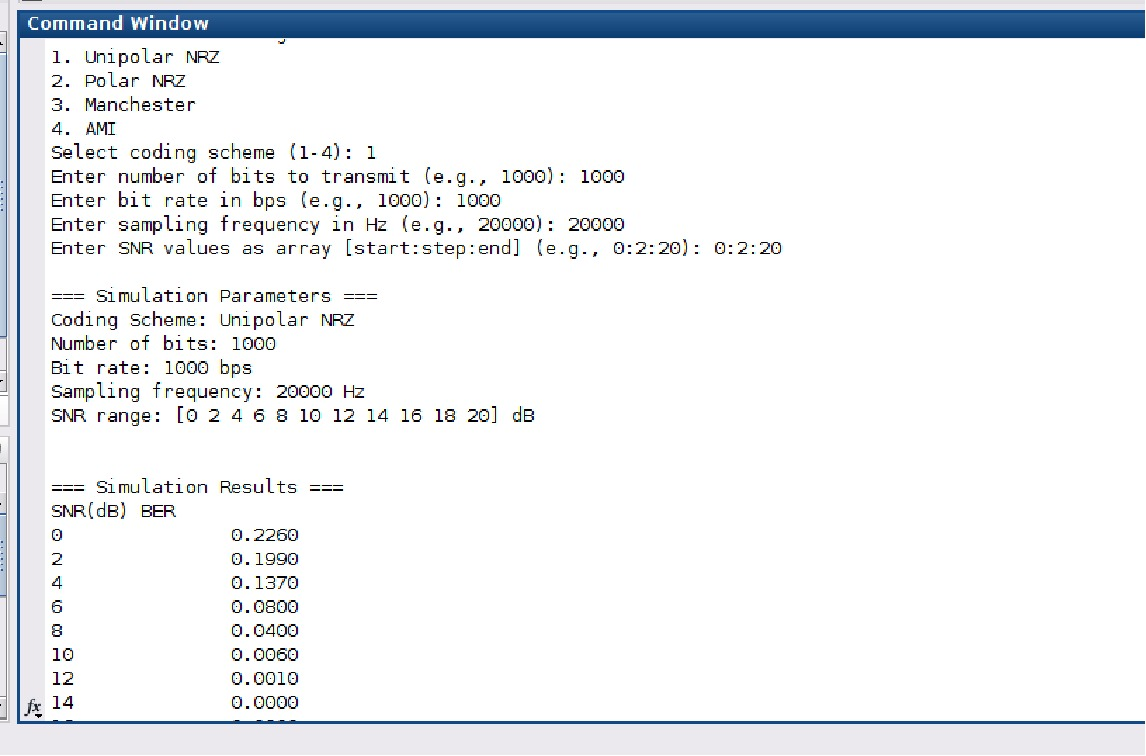
\includegraphics[scale=0.5]{Figures/WhatsApp Image 2025-05-15 at 22.12.46_834d1cda.jpg}

\subsection{Result\_portion\_2}
       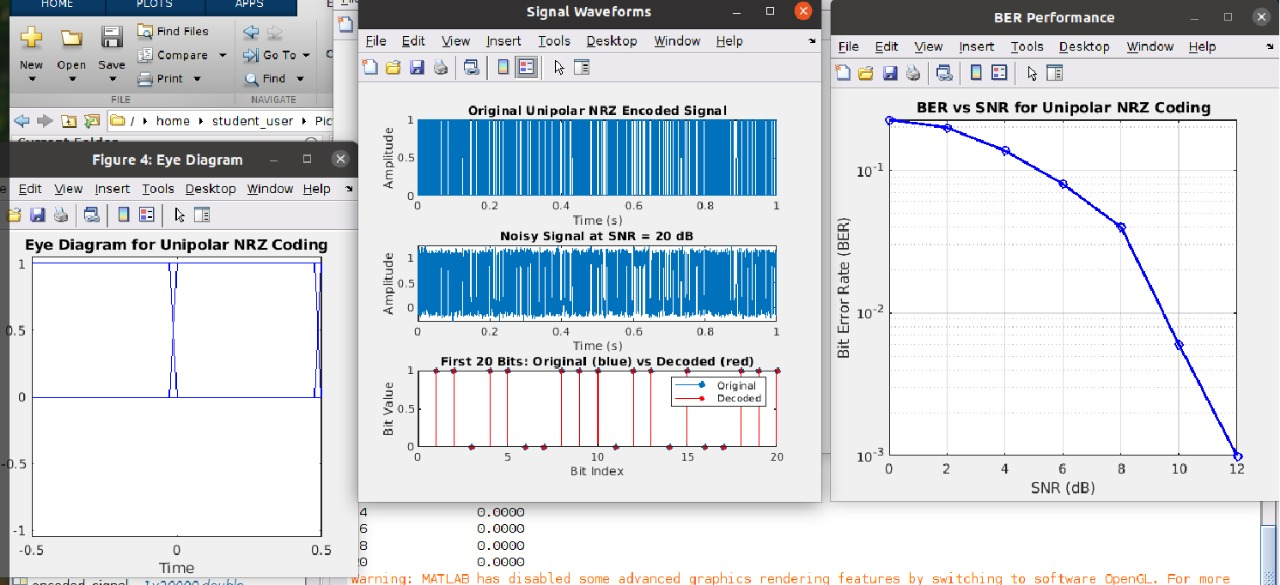
\includegraphics[scale=0.5]{Figures/WhatsApp Image 2025-05-15 at 22.11.02_a23ed3ca.jpg}

\section{Results Overall Discussion}
    
\item 1.Error Increases with Low SNR
When the Signal-to-Noise Ratio (SNR) is low, the simulation shows a high number of errors in the transmitted data. This means noise strongly affects the signal and causes mistakes in decoding.

\item 2.Different Line Codings Perform Differently
Some line coding schemes perform better than others in noisy environments. For example, Manchester and AMI give better results in terms of Bit Error Rate (BER) compared to Unipolar NRZ at the same SNR values.

\item 3.BER Decreases with Higher SNR
As the SNR increases, the BER (Bit Error Rate) becomes lower. This shows that better signal quality helps reduce transmission errors and improves communication reliability.



\end{enumerate}
% Chapter 3 ends here..... 




% Chapter 5 starts here..... 
\newpage
\chapter{Conclusion}

\section{Discussion}

\item This project helped us learn how data is sent using line coding in digital communication. We saw that when data travels, small errors can happen, and even one wrong bit can change the full message.

\item By simulating these errors, we understood why error detection and correction are so important. The project made it easier to see how line coding works and how problems happen during data transmission.

\item It is a very useful project for students to understand the basic idea of data communication and error handling in a simple and practical way.


\end{itemize}

\section{Limitations}

\item .The project supports only a few line coding types (like NRZ, RZ, and Manchester).

\item .It simulates only simple bit errors, not advanced error patterns.

\item .There is no error correction, only error simulation.

\item .The user interface is simple and not graphical.

\end{itemize}
\end{itemize}
 

\section{Scope of Future Work}
\item .Add more line coding techniques (like AMI, B8ZS, HDB3).
\item .Add error detection and correction (like parity check, Hamming code).
\item Create a graphical user interface (GUI) for better visualization.

\item . Use real-time input/output for real-world simulation.


\end{itemize}   
\end{enumerate}


% Chapter 5 ends here..... 




% References starts here..... 
\newpage
  \renewcommand\bibname{References}
  \bibliographystyle{unsrt}
  \bibliography{Ref}
  \begin{itemize}
      
  

  \item https://www.scribd.com/document/615309205/Mini-project-138-45
\end{itemize}
\end{document}